%*****************************************************************************************
%*********************************** First Chapter ***************************************
%*****************************************************************************************

\chapter{Introduction}

\graphicspath{{Chapter1/Figures/}}

Semiconducting behaviour was first reported in the 19th century. Michael Faraday noted in 1839 that the conductivity of silver selenide increased with temperature, opposite to what is expected in a metal \cite{Faraday2012}. In 1839 Alexandre-Edmond Becquerel reported photovoltaic behaviour in silver chloride coated platinum electrodes in an aqueous nitric acid electrolyte, where an increase in the voltage was observed when one electrode was illuminated with sunlight \cite{Becquerel1839}. A photovoltaic cell was produced by Charles Fritts in 1883 using 30\,$\mu$m thick selenium film with thin gold leaf contacts, with efficiency <1\% \cite{Fritts1883}. Photoconductivity was first reported in selenium bars by Willoughby Smith in 1873, showing in the change in resistance as a result of exposure to sunlight \cite{Smith1873}, as well as William Grylls Adams and Richard Evans Day in 1876, who reported the production of electricity in selenium due to an exposure to sunlight \cite{Adams1876}. Electroluminescent behaviour was first reported in SiC by Henry Joseph Round in 1907, who reported emission when a current was passed through crystals \cite{Round1907}. Simple principles such as these underpin the electronic devices we use today, yet it was not until Alan Wilson's work on band theory in 1931 that such behaviour could be understood and explained \cite{Wilson1931}. 

Throughout the 20th century research was focused on using semiconductors for devices, from the developments of rectifiers and diodes in the early part of the century to the first transistor built at Bell Laboratories in 1946 by William Shockley [Fig.\,\ref{1Fig1}(a)], John Bardeen and Walter Brattain using Ge. Much work has been undertaken to refine and improve the design of these devices to the more sophisticated designs used in our devices today, however the efficiency of such devices hinges on the quality of the semiconducting material used, and the ability to control impurities and dopants in the crystal. From the earliest devices using materials such as lead selenide, we now moved on to devices made using Si and Ge, which are still used today.

Si is the most widely used material in the semiconductor industry due to its abundance in the Earth's crust, low unit cost and simple and well-developed processing techniques. Its high band gap gives it thermal stability, allowing it to be used at high operating temperatures. Si is also highly mechanically stable with high electron mobility, and the native oxide insulating layer that spontaneously grows can be useful in electronics. Although Ge has higher conductivity than Si, its lower band gap gives devices more temperature sensitivity so it is less often used in devices. Alloys of Si and Ge may be used to combine the properties of both materials. One of the main disadvantages of Si is its indirect band gap, meaning it is a poor emitter for luminescence devices. However the GaAs has a direct band gap and can be used in luminescent devices, and its high electron mobility and band gap means it can be used in high speed devices. Other alloys, for example between Group III-V or II-VI atoms, can be used to tune the band gap and other optoelectronic properties. Alloys can also be combines to make lower-dimension structures, producing other desirable properites.
\begin{figure}[ht]
\centering
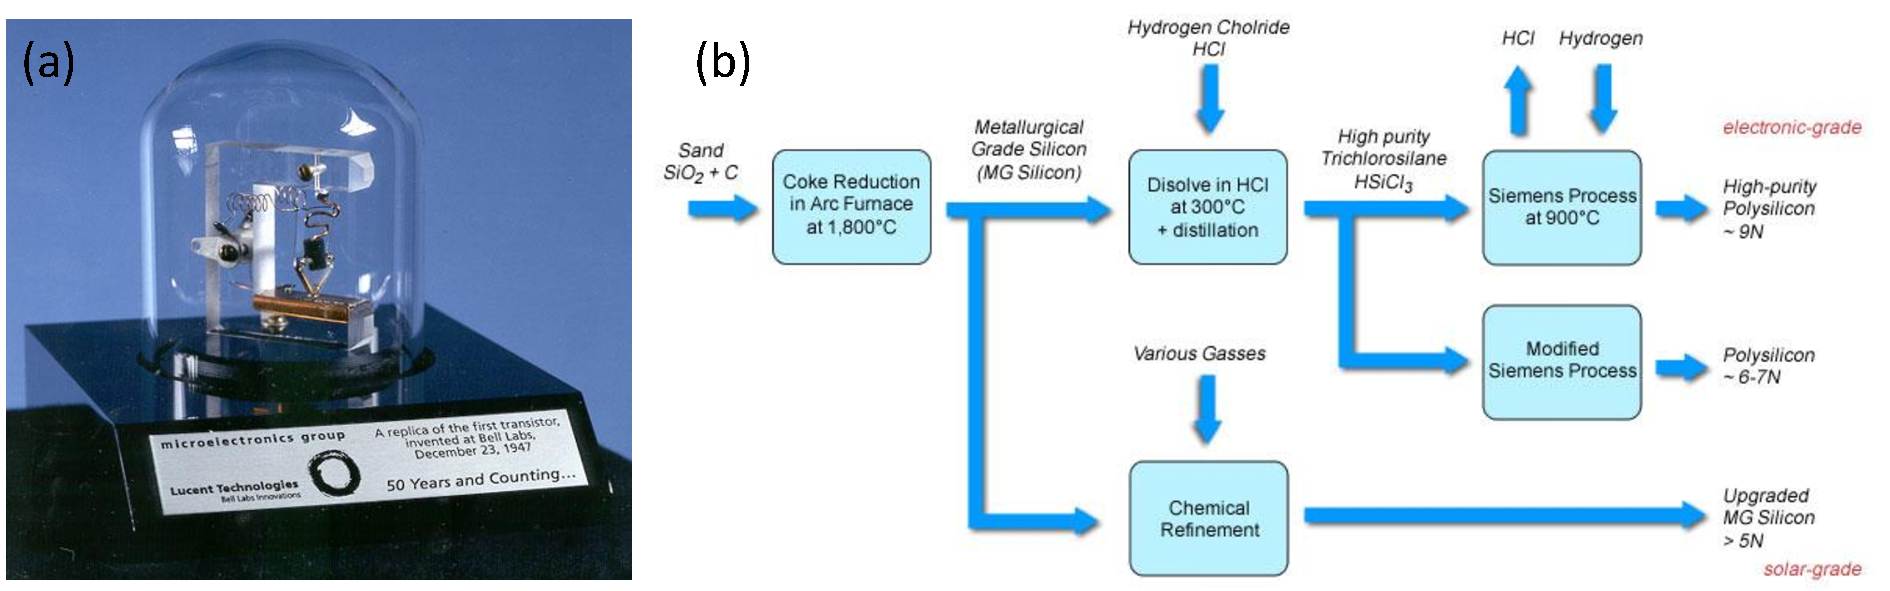
\includegraphics[width=\textwidth]{Fig1}
\caption{(a) Replica of first transistor built in 1946. Reproduced from Ref.\,\cite{Transistor}. (b) Schematic of process required to produce device-grade silicon from starting materials. Reproduced from Ref.\,\cite{Silicon}.}
\label{1Fig1}
\end{figure}

Despite the high stability and carrier mobility in inorganic semiconductors mentioned previous, one major disadvantage is with the processing of such materials. Although Si processing is well-developed, creation of device-grade material still requires many purification steps [Fig.\,\ref{1Fig1}(b)]. Alloys are often produced using vapour or electron-beam deposition, and as such the environmental parameters must be strictly controlled. Layer-by-layer growth can be used for the best quality material, however such processes are costly and time consuming. Current advances in technology require flexible, lightweight and more easily processable semiconductors. 

Although conduction was noted in a mix of aniline and sulphiric acid by Henry Letherby in 1862, research on organic seminconductors began in earnest in the latter half of the 20th century. Polycyclic aromatic compounds were found to form semiconducting charge transfer complexes with halogens in 1954 \cite{Naarmann2002}, and since then much work has been done on developing new molecules and polymers with desired optoelectronic properties, driven by the relative ease with which such molecules can be synthesised. Doping was developed in the 1970s to produce metallic and even superconducting complexes, for example highly conductive oxidised and iodine-doped polyacetylene in 1979 \cite{Shirakawa1977}. Organic semiconductors consist of conjugated molecules, whose overlapping $\pi$ orbitals allow charge transport within the molecule. Given the low production cost, work has be undertaken to produce devices made of organic semiconductors, notably organic photovoltaics, thin film transistors, and light emitting diodes (OLED), probably the most mature organic electronic device as OLEDs have been used mobile phone displays and TVs, with better efficiency and brightness. However problems exist with the manufacturing of such devices, as mass production is not currently optimised for the organic electronic market. More fundamentally, organic semiconductors are less thermally, optically and electrically stable than their inorganic counterparts, leading to lower lifespan of devices. Charge mobility is also lower as hopping between adjacent molecules is required, and lower crystallinity of materials leads to scattering at grain boundaries. 
\begin{figure}[ht]
\centering
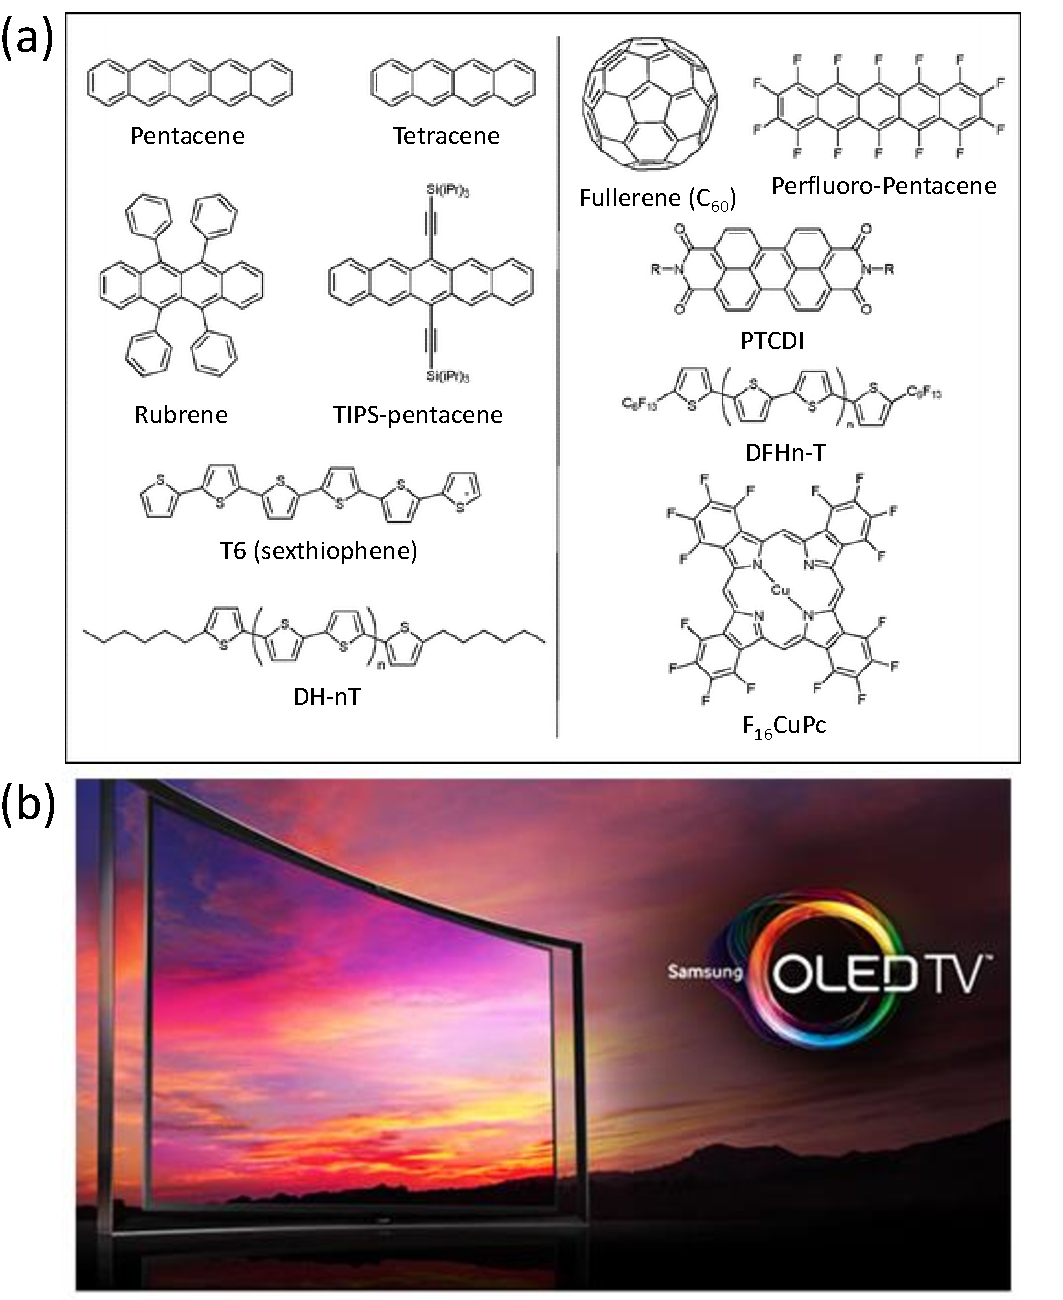
\includegraphics[width=\textwidth]{Fig2}
\caption{(a) Common organic semiconductors, with p-type materials on the left and n-type on the right. Modified from Ref.\,\cite{Miozzo2010}. (b) Samsung curved smart OLED TV. Reproduced from Ref.\,\cite{Samsung}.}
\label{1Fig2}
\end{figure}

A new class of hybrid materials has emerged in the last 20 years. Metal halide based organic-inorganic perovskite semiconductors combine the stability of the inorganic semiconductors with the processability of organic semiconductors. A variety of inorganic frameworks can be formed, all of which are self-assembling. Charge carriers are excited in the inorganic network, and thus share similar optical and electrical properties.

This thesis explores the optical properties of 2D lead iodide-based perovskites, particularly the interactions of perovskite excitons and collective electron oscillations in noble metal nanostructures called surface plasmons. We will first introduce the theory of excitons and review the research on lead iodide perovskites, before exploring the optical properties of surface plasmons. In Chapter 4 we will explore the fabrication of perovskite thin films via spin coating, then study the optical properties of ultra-thin perovskite samples produced via exfoliation in Chapter 5. In Chapter 6 we will explore exciton-localised surface plasmon interactions in perovskite-coated metal island structures. Finally in Chapter 7 we look at the coupling between excitons and surface plasmon polaritons in coated plasmonic gratings.